\section{Ukladanie}

V závere celého procesu vytvárania HDR fotografie musí byť užívateľ schopný uložiť si výsledok. Aplikácia ponúka
uloženie nielen výslednej fotografie v štandardnom obrazovom formáte \texttt{JPEG}, ale aj uloženie HDR obsahu 
pre neskoršiu editáciu. V tomto prípade je HDR obsah komprimovaný kódovaním RGBE, ktorý je popísaný v podkapitole
\ref{section-formats} Formáty HDR obsahu. Uloženie HDR formátu je veľkou výhodou, ktorú neponúka žiadna z aplikácií
prieskumu. Užívateľ sa totiž nemusí práve nachádzať v situácii, kedy si nájde čas na vhodné prispôsobenie výsledných
parametrov LDR obrazu.

Kódovanie HDR obsahu je implementované prostredníctvom modulu \texttt{imgcodecs} knižnice OpenCV, konkrétne funkciou
\texttt{imwrite}. Následné načítanie \texttt{.hdr} súboru sa vykonáva pomocou funkcie \texttt{imread}.
Užívateľ môže k uloženým HDR súborom pristupovať kedykoľvek z domovskej obrazovky aplikácie kliknutím na tlačidlo
"Load". Po zvolení tejto možnosti sa zobrazí obrazovka, ktorá obsahuje výpis (\texttt{ListView}) uložených
\texttt{.hdr} súborov v zariadení užívateľa. Výberom jedného z ponúkaných súborov sa súbor načíta a zobrazí 
sa obrazovka pre editáciu HDR obsahu.

Pri vstupno-výstupných operáciách nad úložiskom zariadenia je potrebné získať cestu typu \texttt{java.io.File}.
Na to slúži trieda \texttt{Storages}, ktorá obsahuje statické metódy pre získanie cesty, vrátane vytvorenia
potrebných priečinkov a kontroly, či daná operácia neprepíše existujúci súbor.

Pri ukladaní HDR obsahu alebo LDR výslednej fotografie je užívateľ pomocou dialógového okna vyzvaný, aby do textového
poľa vložil názov svojho nového súboru (obr. \ref{fig:saveDialog}). Z hľadiska funkcionality, sa vytvorí nová inštancia
triedy \texttt{SaveDialog}, ktorá je rozšírená o funkcionalitu triedy \texttt{DialogFragment}. V metóde \texttt{onCreateDialog}
sa pomocou \texttt{AlertDialog.Builder} vytvoria komponenty rozhrania dialógového okna. Príponu ukladaného súboru nevolí
užívateľ, ale je zvolená aplikáciou podľa formátu, v akom bude súbor uložený.

\begin{figure}[h!]
  \centering
  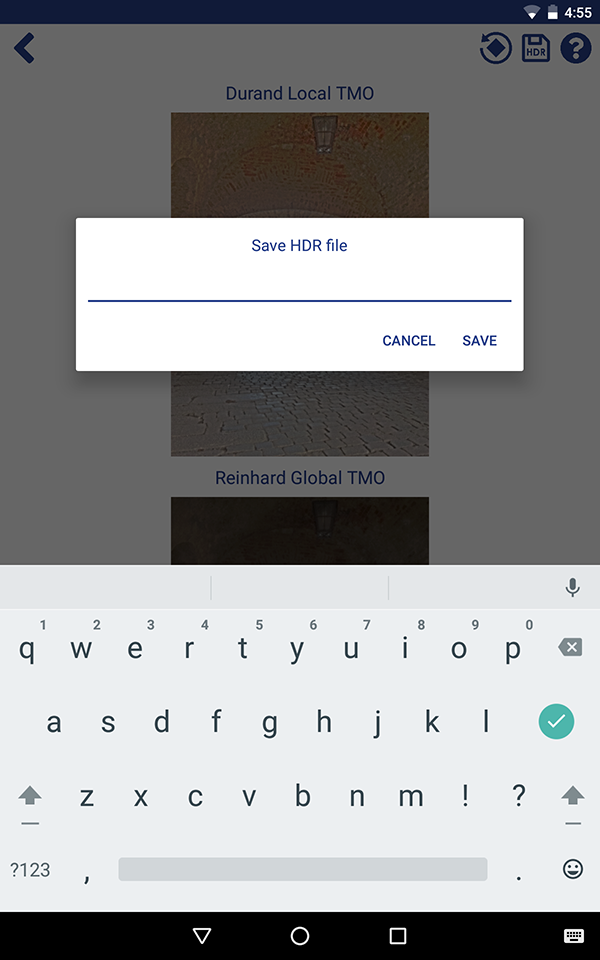
\includegraphics[width=0.35\textwidth]{figures/storage/dialogs/saveHdr}
  % 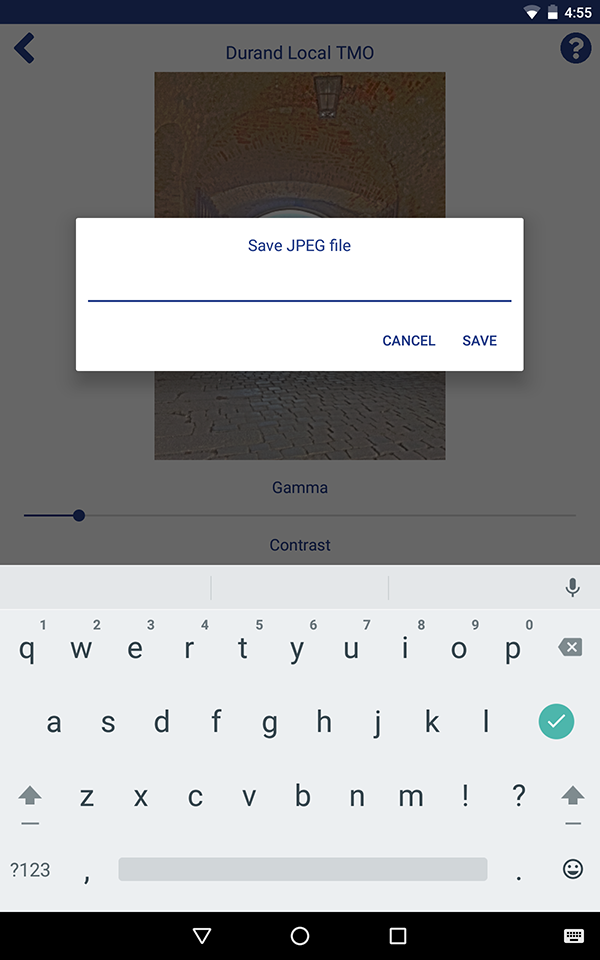
\includegraphics[width=0.3\textwidth]{figures/storage/dialogs/saveJpeg}
  \caption{Dialógové okno pre uloženie súboru vo formáte \texttt{.hdr}}
  \label{fig:saveDialog}
\end{figure}

\subsection*{Úložiská Android zariadenia}

Systém Android ponúka niekoľko možností pre uloženie dát aplikácie. Výber závisí od pot-rieb aplikácie, napríklad
od objemu dát alebo od prístupnosti dát iným aplikáciám. Dos-tupné možnosti uloženia dát v zariadení sú \cite{Android}:
\begin{itemize}
  \item Interné úložisko zariadenia - privátne súbory aplikácie v zariadení.
  \item Externé úložisko zariadenia - zdieľaný súborový systém zariadenia.
  \item Lokálne úložisko - ukladanie neobjemných dát typu kľúč, hodnota.
  \item Databázy - uloženie štruktúrovaných údajov do súkromnej SQLite databázy.
\end{itemize}

Pre ukladanie dát aplikácie je využité externé úložisko. Toto úložisko je vhodným miestom pre súbory, ktoré
nevyžadujú ombedzenia prístupu a pre súbory, ktoré majú byť zdieľané s inými aplikáciami alebo viditeľné pri
prenose súborov do počítača. Výsledné HDR fotografie by mali byť prístupné aj pre iné aplikácie v zariadení
a súbory formátu \texttt{.hdr} môžu vyžadovať viac pamäte, preto je ich vhodné ukladať do externého úložiska. 
Externé úložisko nemusí byť stále k~dispozícii, keďže môže byť obsiahnuté na úložnom médiu ako napríklad SD karte.
Aplikácii, pracujúcej s externým úložiskom, musia byť užívateľom udelené povolenia \texttt{WRITE\_EXTERNAL\_STORAGE} 
a \texttt{READ\_EXTERNAL\_STORAGE}.

V prípade, ak by aplikácia ukladala krivku odozvy fotoaparátu, ktorá je špecifická pre snímač zariadenia, dáta
by sa uložili na interné úložisko. Interné úložisko zariadenia je k~dispozícii nepretržite. Súbor je prístupný
iba danej aplikácii a po odinštalovaní aplikácie systém odstráni všetky súbory aplikácie z interného úložiska.